\section{Examples of dynamics on abelian varieties}

On this section, fix an algebraically closed field \(\kkk\) of characteristic zero.
Everything is defined over \(\kkk\) unless otherwise specified. 

\subsection{Product of elliptic curves}

    In this subsection, we consider the dynamics induced by matrices on the product of elliptic curves.

    % \begin{example}\label{eg:dynamics_induced_by_matrix_on_product_of_elliptic_curves}
    Let \(E\) be an elliptic curve without complex multiplication. 
    Consider the abelian variety \(X = E \times E\). 
    Let \(f_A: X \to X\) be the endomorphism defined by the matrix
    \[ A = \begin{pmatrix}
        a & b \\
        c & d
    \end{pmatrix}. \]
    Let \([F_1], [F_2], [\Delta]\) be the classes of the fibers of the two projections and the diagonal in \(\NS(X)\).
    It is well-known that they span \(\NS(X)\) and the intersection numbers are given by
    \[ [F_1]^2 = [F_2]^2 = [\Delta]^2 = 0, \quad [F_1] \cdot [F_2] = [F_1] \cdot [\Delta] = [F_2] \cdot [\Delta] = 1; \]
    see \cite[Section 1.5.B]{Laz04a}.

    We have that \(f_A^*[F_1]\) is given by \([a]_E (x) + [b]_E (y) = 0\).
    Then 
    \[ f_A^*[F_1].[F_1] = b^2, \quad f_A^*[F_1].[F_2] = a^2, \quad f_A^*[F_1].[\Delta] = (a+b)^2. \]
    Hence 
    \[ f_A^*[F_1] = (a^2+ab) [F_1] + (b^2+ab) [F_2] - ab [\Delta]. \]
    Similarly, we have
    \begin{align*}
        f_A^*[F_2] &= (c^2+cd) [F_1] + (d^2+cd) [F_2] - cd [\Delta], \\
        f_A^*[\Delta] &= (a-c)(a+b-c-d) [F_1] + (b-d)(a+b-c-d) [F_2] - (a-c)(b-d) [\Delta].
    \end{align*}
    Thus, the matrix representation of \(f_A^*\) on \(\NS(X)\) with respect to the basis \(\{[F_1], [F_2], [\Delta]\}\) is
    \[
        \begin{pmatrix}
            a^2+ab & c^2+cd & (a-c)(a+b-c-d) \\
            b^2+ab & d^2+cd & (b-d)(a+b-c-d) \\
            -ab & -cd & -(a-c)(b-d)
        \end{pmatrix}.
    \]

    If we take \(e_1= [F_1],e_2=[F_2],e_3=[\Delta]-[F_1]-[F_2]\) as a new basis of \(\NS(X)\), then the matrix representation of \(f_A^*\) on \(\NS(X)\) with respect to the basis \(\{e_1,e_2,e_3\}\) is
    \[
        M = \begin{pmatrix}
            a^2 & c^2 & -2ac \\
            b^2 & d^2 & -2bd \\
            -ab & -cd & ad+bc
        \end{pmatrix}.
    \]
    The characteristic polynomial of \(M\) is given by
    \[ \chi_{f_A^*}(T) = (T - (ad-bc))(T^2 - (a^2+d^2+2bc)T + (ad-bc)^2). \]
    Suppose that the eigenvalues of \(A\) are \(\lambda, \mu\).
    Then the eigenvalues of \(f_A^*\) on \(\NS(X)\) are given by \(\lambda^2, \mu^2, \lambda \nu\).
    When \(a-d,b,c\) are not all zero, \(\NS(X)\) has two invariant subspaces of dimension \(1\) and \(2\) respectively.
    They are given by 
    \[ V_1 = \bbQ \cdot \begin{pmatrix}
        2c \\
        -2b \\
        a-d
    \end{pmatrix}, \quad V_2 = \bbQ \cdot \begin{pmatrix}
        0 \\
        a-d \\
        c
    \end{pmatrix} \oplus \bbQ \cdot \begin{pmatrix}
        d-a \\
        0 \\
        b
    \end{pmatrix} = \{(p,q,r) \mid bp-cq+(a-d)r=0\}. \]
    with respect to the basis \(\{e_i\}\).
    One can use \cref{code:matrix_representation_of_dynamics_on_product_of_elliptic_curves} to check this in \href{https://sagecell.sagemath.org/}{SageMathCell}.

    With respect to the basis \(\{e_i\}\), the cones are given by
    \[ \Nef(X) = \Psef(X) = \{p e_1 + q e_2 + r e_3 \mid p,q \geq 0, \quad pq \geq r^2\}. \]
    We analyze the intersection of \(V_1, V_2\) with \(\Psef(X)\).
    On the plane \(P: p+q = 2\), fix a coordinate system \((s,r)\) with \(s = (p-q)/2 = p-1 = 1-q\).
    The cone \(\Psef(X)\) is given by the disk \(\{ (s,r) \mid s^2 + r^2 \leq 1\}\).
    The plane \(V_2\) is given by the equation \(b(1+s) - c(1-s) + (a-d)r = (b-c) + (b+c)s + (a-d)r = 0\).
    If \(b=c\), then the line \(V_1\) does not intersect the plane \(P\), hence does not intersect the interior of \(\Psef(X)\).
    Otherwise, \(V_1 \cap P\) is given by the point \((s,r) = \left(\frac{c+b}{c-b}, \frac{a-d}{c-b}\right)\).
    There are three cases:
    \begin{enumerate}
        \item \((a+d)^2 < 4(ad-bc)\): \(V_1\) intersects the interior of \(\Psef(X)\), \(V_2\) intersects \(\Psef(X)\) at only the origin.
        \item \((a+d)^2 = 4(ad-bc)\): \(V_1\) intersects the boundary of \(\Psef(X)\) at a ray, \(V_2\) intersects the boundary of \(\Psef(X)\) at a ray.
        \item \((a+d)^2 > 4(ad-bc)\): \(V_1\) intersects \(\Psef(X)\) at only the origin, \(V_2\) intersects the interior of \(\Psef(X)\).
    \end{enumerate}
    Note that if \(b=c\), we always have \((a+d)^2 > 4(ad-bc)\) under the assumption that \(a-d,b,c\) are not all zero.
    And note that \((a+d)^2 - 4(ad-bc) = \disc(\chi_A)\).
    Hence, we have the conclusion in \cref{table:intersection_of_invariant_subspaces_with_psef_cone_on_product_of_elliptic_curves}.
    \begin{table}[!ht]
        \centering
        \begin{tabular}{|c|c|c|c|}
            \hline
            Case & $V_1 \cap \Psef(X)$ & $V_2 \cap \Psef(X)$ & \makecell[c]{dimension of minimal \\ invariant subspace \\ intersecting \(\Psef(X)^\circ\)} \\
            \hline
            \(A\) is scalar &  &  &  \\
            \(A\) has only one eigenvalue  & Boundary (ray) & Boundary (ray) & 3 \\
            \(A\) has complex eigenvalues & Interior & Origin only & 1 \\
            \(A\) has distinct real eigenvalues & Origin only & Interior & 2 \\
            \hline
        \end{tabular}
        \caption{Intersection of invariant subspaces $V_1$, $V_2$ with $\Psef(X)$ in different cases.}
        \label{table:intersection_of_invariant_subspaces_with_psef_cone_on_product_of_elliptic_curves}
    \end{table}
        
    Now we focus on the case when \(A\) has only one eigenvalue, i.e. \(A\) is similar to a Jordan block.
    Assume that \(A\) is not a scalar matrix, i.e. \(a-d,b,c\) are not both zero.
    Then easily see that \(V_1 \subset V_2\) iff \((a+d)^2 = 4(ad-bc)\) iff \(A\) has the Jordan normal form \(\begin{pmatrix}
        \lambda & 1 \\
        0 & \lambda
    \end{pmatrix}\) for some \(\lambda \in \bbZ\).
    Hence in this case, there is a finite equivariant cover \((X,f) \to (X,g)\) such that \(g\) is induced by the Jordan block.

    \begin{example}\label{eg:Jordan_block_acts_on_NS_by_endomorphism_of_product_of_elliptic_curves}
        Let \(f: X \to X\) be the endomorphism defined by the matrix
        \[ A = \begin{pmatrix}
            2 & 1 \\
            0 & 2
        \end{pmatrix}. \]
        Then the matrix representation of \(f^*\) on \(\NS(X)\) with respect to the basis \(\{e_1, e_2, e_3\}\) is
        \[
            M = \begin{pmatrix}
                4 & 0 & 0 \\
                1 & 4 & -4 \\
                -2 & 0 & 4
            \end{pmatrix}. 
        \]
        The Jordan normal form of \(M\) is
        \[
            \begin{pmatrix}
                4 & 1 & 0 \\
                0 & 4 & 1 \\
                0 & 0 & 4
            \end{pmatrix}.
        \]
        The invariant subspaces of \(M\) are given by
        \[ V_1 = \bbR \cdot \begin{pmatrix}
            0 \\
            -2 \\
            0
        \end{pmatrix}, \quad V_2 = \{(p,q,r) \mid p = 0\}. \]
        We have \(V_2 \cap \Psef(X) = V_1 \cap \Psef(X) = \bbR_{\geq 0} \cdot (0,1,0)^T\).
        The action of \(f^*\) on \(\NS(X)\) induces a dynamics on the plane \(P: p+q=2\); see \cref{fig:dynamics_on_NS_of_product_of_elliptic_curves_Jordan_block}.
    \end{example}
    \begin{figure}[!ht]
        \centering
        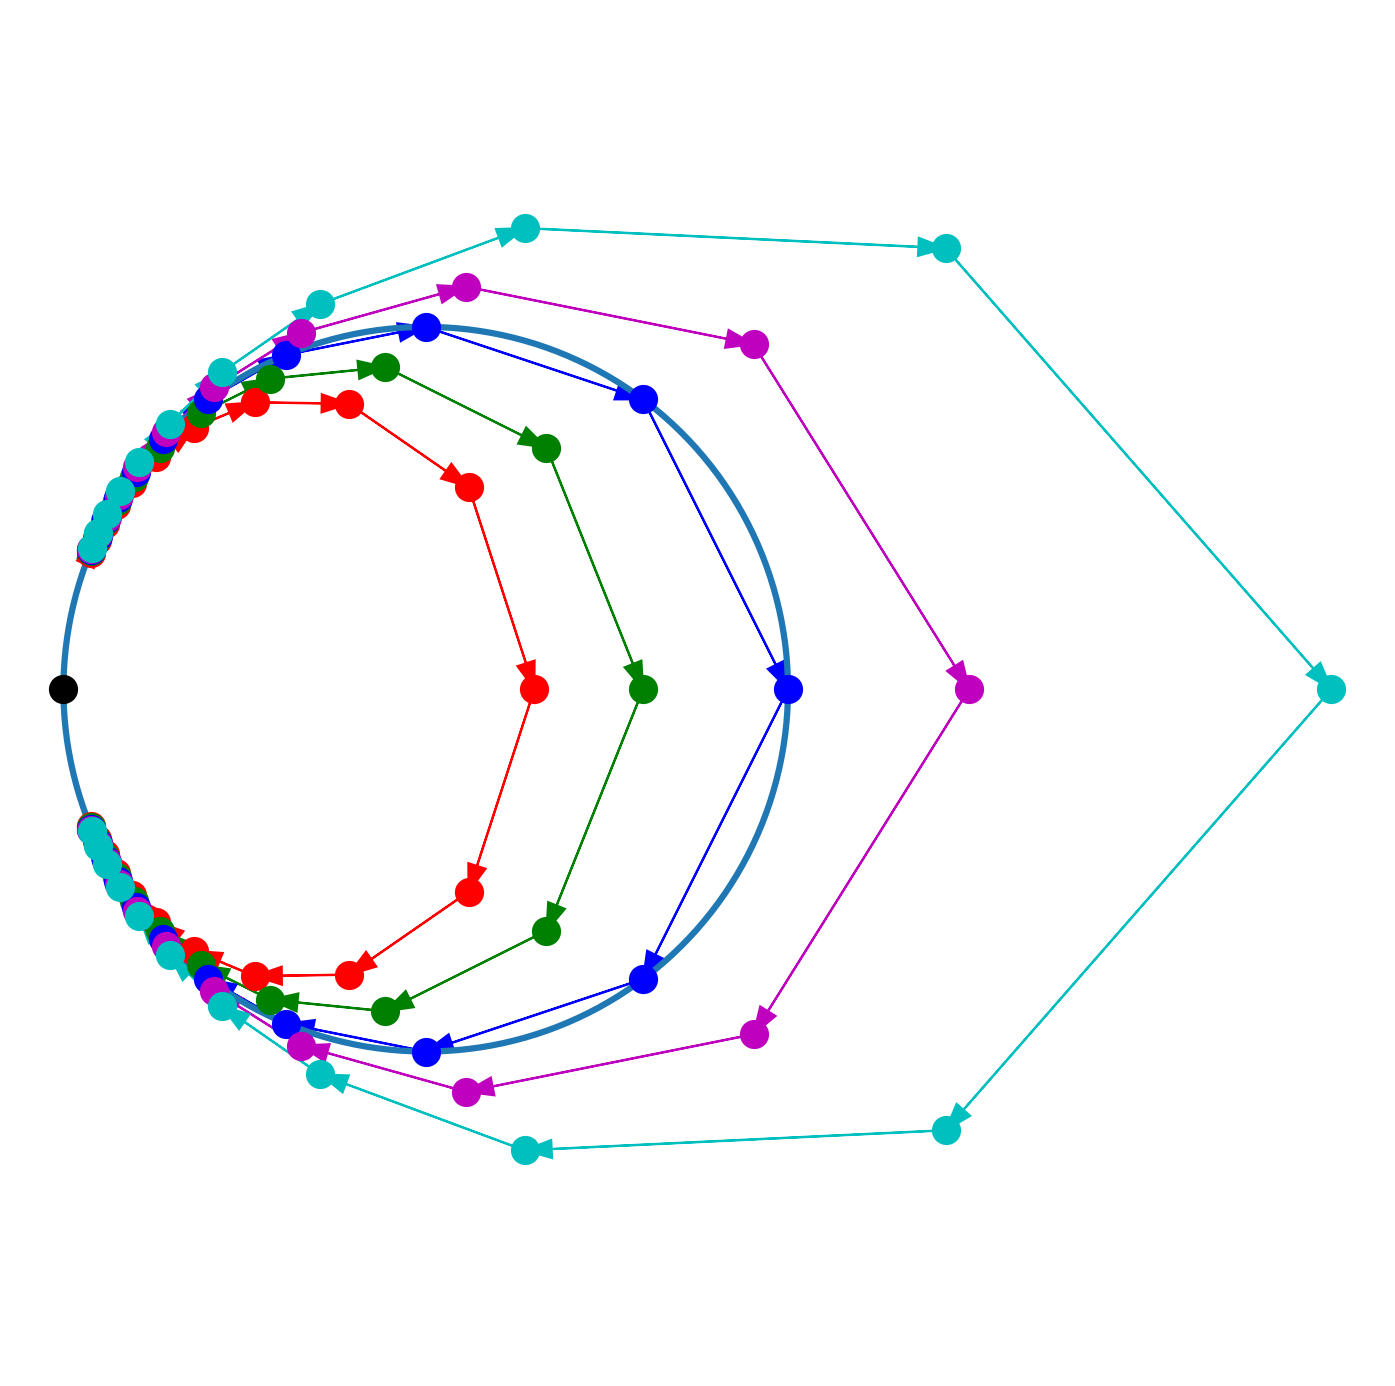
\includegraphics[width=0.3\textwidth]{jordan_block_action_plot_product_of_elliptic_curve.png}
        \caption{Dynamics on \(\NS(X)\) induced by the endomorphism defined by a Jordan block.}
        \label{fig:dynamics_on_NS_of_product_of_elliptic_curves_Jordan_block}
    \end{figure}




    \subsection{Appendix}
        
        \lstinputlisting[language=Python, caption={Test invariant subspaces of \(\NS(E\times E)\)}, label=code:matrix_representation_of_dynamics_on_product_of_elliptic_curves]{matrix_representation_of_dynamics_on_E_times_E.sage}

